\documentclass[a4paper]{book}
\usepackage{makeidx}
\usepackage{graphicx}
\usepackage{multicol}
\usepackage{float}
\usepackage{listings}
\usepackage{color}
\usepackage{ifthen}
\usepackage[table]{xcolor}
\usepackage{textcomp}
\usepackage{alltt}
\usepackage[utf8]{inputenc}
\usepackage[spanish]{babel}
\usepackage{mathptmx}
\usepackage[scaled=.90]{helvet}
\usepackage{courier}
\usepackage{doxygen}
\lstset{language=C++,inputencoding=utf8,basicstyle=\footnotesize,breaklines=true,breakatwhitespace=true,tabsize=8,numbers=left }
\makeindex
\setcounter{tocdepth}{3}
\renewcommand{\footrulewidth}{0.4pt}
\begin{document}
\begin{titlepage}
\vspace*{7cm}
\begin{center}
{\Large is2010final \\[1ex]\large 1 }\\
\vspace*{1cm}
{\large Generado por Doxygen 1.7.2}\\
\vspace*{0.5cm}
{\small Lunes, 1 de Noviembre de 2010 22:59:10}\\
\end{center}
\end{titlepage}
\clearemptydoublepage
\pagenumbering{roman}
\tableofcontents
\clearemptydoublepage
\pagenumbering{arabic}
\chapter{Página principal}
\label{index}\begin{center}{\bfseries Proyecto de Ingenieria de Software 2010}\end{center}  \par


Relaciones entre clases por medio de un diagrama de lineas de dot: \begin{center}

\begin{DoxyImageNoCaption}
  \mbox{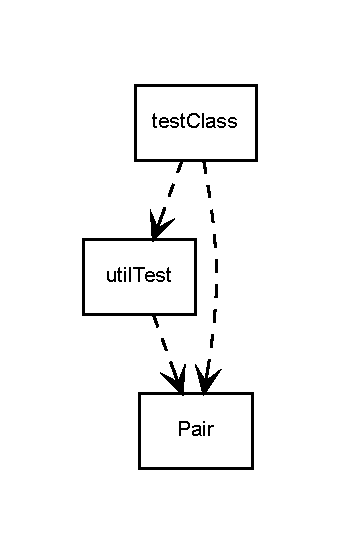
\includegraphics[width=\textwidth]{inline_dotgraph_1}}
\end{DoxyImageNoCaption}
\end{center}
 Nota: las clases en el grafico son clickables (en salida HTML).

\begin{DoxyAuthor}{Autor}
BERNAL, Matias\par
 BRESSAN, Gonzalo\par
 JAULE, Marcos\par
 ODORIZZI, Eduardo
\end{DoxyAuthor}
\par
 \begin{center} \end{center}  \par
 {\tt Repositorio SVN en Google Code} 
\chapter{Índice de clases}
\section{Class List}
Here are the classes, structs, unions and interfaces with brief descriptions:\begin{DoxyCompactList}
\item\contentsline{section}{\hyperlink{classutil_1_1_pair}{util.Pair} (La clase pair implementa el tipo Par )}{\pageref{classutil_1_1_pair}}{}
\item\contentsline{section}{\hyperlink{classtest_1_1test_class}{test.testClass} (La clase \hyperlink{classtest_1_1test_class}{testClass} declara una serie de metodos en jUnit\par
 para verficar el correcto funcionamiento de las funciones de validacion\par
 de la clase utilTest.\par
 )}{\pageref{classtest_1_1test_class}}{}
\item\contentsline{section}{\hyperlink{classutil_1_1util_test}{util.utilTest} (La clase \hyperlink{classutil_1_1util_test}{utilTest} declara una serie de metodos para realizar validaciones de, entre otros,\par
 Cadenas, Fechas, Tiempo transcurrido )}{\pageref{classutil_1_1util_test}}{}
\end{DoxyCompactList}

\chapter{Indice de archivos}
\section{File List}
Here is a list of all documented files with brief descriptions:\begin{DoxyCompactList}
\item\contentsline{section}{src/test/\hyperlink{test_class_8java}{testClass.java} (Este archivos contiene la implementacion de las pruebas )}{\pageref{test_class_8java}}{}
\item\contentsline{section}{src/util/\hyperlink{_pair_8java}{Pair.java} (Este archivo contiene la impementaci\'{o}n del tipo Par )}{\pageref{_pair_8java}}{}
\item\contentsline{section}{src/util/\hyperlink{util_test_8java}{utilTest.java} (This file contains the DoxygenExample class with the main() function )}{\pageref{util_test_8java}}{}
\end{DoxyCompactList}

\chapter{Documentación de las clases}
\section{Referencia de la Clase util.Pair}
\label{classutil_1_1_pair}\index{util::Pair@{util::Pair}}


La clase pair implementa el tipo Par.  


\subsection*{Métodos públicos}
\begin{DoxyCompactItemize}
\item 
{\bf Pair} ()\label{classutil_1_1_pair_a9d7967397137600f7a78b7c5b0366050}

\begin{DoxyCompactList}\small\item\em constructor sin parametros \par
 crea el par (0,0). \item\end{DoxyCompactList}\item 
{\bf Pair} (int x, int y)
\begin{DoxyCompactList}\small\item\em constructor con parametros \par
 crea el par (x,y). \item\end{DoxyCompactList}\item 
int {\bf getX} ()
\begin{DoxyCompactList}\small\item\em devuelve la primer componente del par. \item\end{DoxyCompactList}\item 
void {\bf setX} (int x)
\item 
int {\bf getY} ()
\begin{DoxyCompactList}\small\item\em devuelve la segunda componente del par. \item\end{DoxyCompactList}\item 
void {\bf setY} (int y)
\end{DoxyCompactItemize}


\subsection{Descripción detallada}
La clase pair implementa el tipo Par. El tipo par representa dos n�meros escritos en un cierto orden.\par
 Usualmente est�n escritos entre par�ntesis, as�: (4,5) 

\subsection{Documentación del constructor y destructor}
\index{util::Pair@{util::Pair}!Pair@{Pair}}
\index{Pair@{Pair}!util::Pair@{util::Pair}}
\subsubsection[{Pair}]{\setlength{\rightskip}{0pt plus 5cm}util.Pair.Pair (
\begin{DoxyParamCaption}
\item[{int}]{ x, }
\item[{int}]{ y}
\end{DoxyParamCaption}
)}\label{classutil_1_1_pair_a72710069b672dfd62f8bbc6cadb799f8}


constructor con parametros \par
 crea el par (x,y). 


\begin{DoxyParams}{Parámetros}
{\em x} & primer valor del par. \\
\hline
{\em y} & segungo valor del par. \\
\hline
\end{DoxyParams}


\subsection{Documentación de las funciones miembro}
\index{util::Pair@{util::Pair}!getX@{getX}}
\index{getX@{getX}!util::Pair@{util::Pair}}
\subsubsection[{getX}]{\setlength{\rightskip}{0pt plus 5cm}int util.Pair.getX (
\begin{DoxyParamCaption}
{}
\end{DoxyParamCaption}
)}\label{classutil_1_1_pair_a350e02bc8be591f0e4287874b57effc0}


devuelve la primer componente del par. 

\begin{DoxyReturn}{Devuelve}
x 
\end{DoxyReturn}
\index{util::Pair@{util::Pair}!getY@{getY}}
\index{getY@{getY}!util::Pair@{util::Pair}}
\subsubsection[{getY}]{\setlength{\rightskip}{0pt plus 5cm}int util.Pair.getY (
\begin{DoxyParamCaption}
{}
\end{DoxyParamCaption}
)}\label{classutil_1_1_pair_af550353978249bacbbd1eed10890ed88}


devuelve la segunda componente del par. 

\begin{DoxyReturn}{Devuelve}
y 
\end{DoxyReturn}
\index{util::Pair@{util::Pair}!setX@{setX}}
\index{setX@{setX}!util::Pair@{util::Pair}}
\subsubsection[{setX}]{\setlength{\rightskip}{0pt plus 5cm}void util.Pair.setX (
\begin{DoxyParamCaption}
\item[{int}]{ x}
\end{DoxyParamCaption}
)}\label{classutil_1_1_pair_af9821418435f2417364781fe92456da6}
setea la primer componente del par. 
\begin{DoxyParams}{Parámetros}
{\em x} & \\
\hline
\end{DoxyParams}
\index{util::Pair@{util::Pair}!setY@{setY}}
\index{setY@{setY}!util::Pair@{util::Pair}}
\subsubsection[{setY}]{\setlength{\rightskip}{0pt plus 5cm}void util.Pair.setY (
\begin{DoxyParamCaption}
\item[{int}]{ y}
\end{DoxyParamCaption}
)}\label{classutil_1_1_pair_a50fb983bf0b28bb19a64484bbc9f2e57}
setea la segunda componente del par. 
\begin{DoxyParams}{Parámetros}
{\em y} & \\
\hline
\end{DoxyParams}


La documentación para esta clase fue generada a partir del siguiente fichero:\begin{DoxyCompactItemize}
\item 
src/util/{\bf Pair.java}\end{DoxyCompactItemize}

\hypertarget{classutil_1_1util_test}{
\section{util.utilTest Class Reference}
\label{classutil_1_1util_test}\index{util::utilTest@{util::utilTest}}
}


La clase \hyperlink{classutil_1_1util_test}{utilTest} declara una serie de metodos para realizar validaciones de, entre otros,\par
 Cadenas, Fechas, Tiempo transcurrido.  


\subsection*{Static Public Member Functions}
\begin{DoxyCompactItemize}
\item 
static boolean \hyperlink{classutil_1_1util_test_a0511fb76ddd99ce9c98231108be97d5a}{checkString} (String s)
\begin{DoxyCompactList}\small\item\em checkString Metodo que verifica si un String pasado como parametro es valido o no. Un string es valido si solo contiene caracteres de a-\/z o de A-\/Z y ademas si su longitid esta entre 1 y 60. \item\end{DoxyCompactList}\item 
static boolean \hyperlink{classutil_1_1util_test_a2c5fbf1f9fb195eb5ff80229cc99c394}{checkDni} (String dni)
\item 
static boolean \hyperlink{classutil_1_1util_test_af38bbc6684ef93d7cd3580df593b1e6a}{checkDate} (int diaA, int mes, int anio)
\item 
static int \hyperlink{classutil_1_1util_test_aaa8556f9ef98f63b750e50af6c3484d1}{hourDiff} (int diaE, int mesE, int anioE, int hsE, int minE, int diaS, int mesS, int anioS, int hsS, int minS)
\item 
static float \hyperlink{classutil_1_1util_test_a991f47fa2395bca0ddc28abb2ca2950f}{medicPay} (Vector$<$ \hyperlink{classutil_1_1_pair}{Pair} $>$ consultas, float valor, int horasAlquiler, float alquilerxhs)
\item 
static float \hyperlink{classutil_1_1util_test_a525d627e3d989ff9190a69fe6bccffff}{totalPay} (Float costoDia, \hyperlink{classutil_1_1_pair}{Pair}\mbox{[}$\,$\mbox{]} comidas, Vector$<$ \hyperlink{classutil_1_1_pair}{Pair} $>$ medicamentos, int dias, Float descuento)
\item 
static int \hyperlink{classutil_1_1util_test_a9e7d593af72519ead8d188becaa1c671}{daysDiff} (int diaE, int mesE, int anioE, int hsE, int minE, int diaS, int mesS, int anioS, int hsS, int minS)
\item 
static boolean \hyperlink{classutil_1_1util_test_a778f4f1a2c59966aa2aae9011bde2ca8}{checkHour} (int hs, int min)
\end{DoxyCompactItemize}


\subsection{Detailed Description}
La clase \hyperlink{classutil_1_1util_test}{utilTest} declara una serie de metodos para realizar validaciones de, entre otros,\par
 Cadenas, Fechas, Tiempo transcurrido. 

\subsection{Member Function Documentation}
\hypertarget{classutil_1_1util_test_af38bbc6684ef93d7cd3580df593b1e6a}{
\index{util::utilTest@{util::utilTest}!checkDate@{checkDate}}
\index{checkDate@{checkDate}!util::utilTest@{util::utilTest}}
\subsubsection[{checkDate}]{\setlength{\rightskip}{0pt plus 5cm}static boolean util.utilTest.checkDate (
\begin{DoxyParamCaption}
\item[{int}]{ diaA, }
\item[{int}]{ mes, }
\item[{int}]{ anio}
\end{DoxyParamCaption}
)\hspace{0.3cm}{\ttfamily  \mbox{[}static\mbox{]}}}}
\label{classutil_1_1util_test_af38bbc6684ef93d7cd3580df593b1e6a}
checkDate valida que la fecha ingresada sea correcta.\par
 una fecha es correcta si el dia es menor que 28 para el mes 2 o 29 en caso de que el a�o sea bisiesto.\par
 el dia es menor o igual que 30 para los meses: 1, 3, 5, 7, 8, 10 y 12\par
 o el dia es menor o igual que 31 para los meses: 4, 6, 9 y 11. 
\begin{DoxyParams}{Parameters}
{\em diaA} & \\
\hline
{\em mes} & \\
\hline
{\em anio} & \\
\hline
\end{DoxyParams}
\begin{DoxyReturn}{Returns}
true si es valido, false si no lo es 
\end{DoxyReturn}


Here is the caller graph for this function:
\nopagebreak
\begin{figure}[H]
\begin{center}
\leavevmode
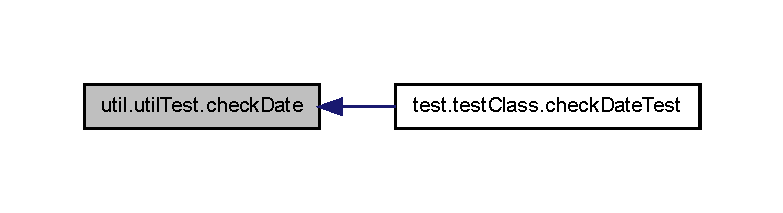
\includegraphics[width=376pt]{classutil_1_1util_test_af38bbc6684ef93d7cd3580df593b1e6a_icgraph}
\end{center}
\end{figure}


\hypertarget{classutil_1_1util_test_a2c5fbf1f9fb195eb5ff80229cc99c394}{
\index{util::utilTest@{util::utilTest}!checkDni@{checkDni}}
\index{checkDni@{checkDni}!util::utilTest@{util::utilTest}}
\subsubsection[{checkDni}]{\setlength{\rightskip}{0pt plus 5cm}static boolean util.utilTest.checkDni (
\begin{DoxyParamCaption}
\item[{String}]{ dni}
\end{DoxyParamCaption}
)\hspace{0.3cm}{\ttfamily  \mbox{[}static\mbox{]}}}}
\label{classutil_1_1util_test_a2c5fbf1f9fb195eb5ff80229cc99c394}
checkDni metodo que verifica si un String pasado como parametro representando un dni es valido o no. Un dni es valido si cumple con la mascara XX.XXX.XXX donde X debe ser un numero de 0-\/9 
\begin{DoxyParams}{Parameters}
{\em String} & s es el string a verificar. \\
\hline
\end{DoxyParams}
\begin{DoxyReturn}{Returns}
boolean true si es valido y false en caso contrario. 
\end{DoxyReturn}


Here is the caller graph for this function:
\nopagebreak
\begin{figure}[H]
\begin{center}
\leavevmode
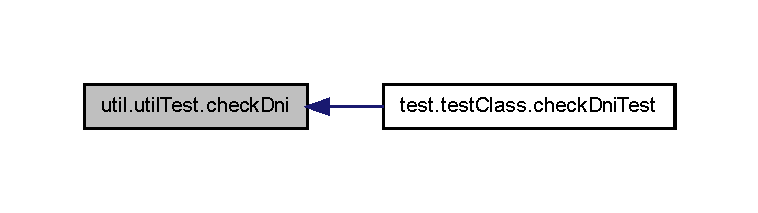
\includegraphics[width=364pt]{classutil_1_1util_test_a2c5fbf1f9fb195eb5ff80229cc99c394_icgraph}
\end{center}
\end{figure}


\hypertarget{classutil_1_1util_test_a778f4f1a2c59966aa2aae9011bde2ca8}{
\index{util::utilTest@{util::utilTest}!checkHour@{checkHour}}
\index{checkHour@{checkHour}!util::utilTest@{util::utilTest}}
\subsubsection[{checkHour}]{\setlength{\rightskip}{0pt plus 5cm}static boolean util.utilTest.checkHour (
\begin{DoxyParamCaption}
\item[{int}]{ hs, }
\item[{int}]{ min}
\end{DoxyParamCaption}
)\hspace{0.3cm}{\ttfamily  \mbox{[}static\mbox{]}}}}
\label{classutil_1_1util_test_a778f4f1a2c59966aa2aae9011bde2ca8}
checkHour comprueba que la hora pasada como parametro es correcta\par
 
\begin{DoxyParams}{Parameters}
{\em hs} & hora \\
\hline
{\em min} & minutos \\
\hline
\end{DoxyParams}


Here is the caller graph for this function:
\nopagebreak
\begin{figure}[H]
\begin{center}
\leavevmode
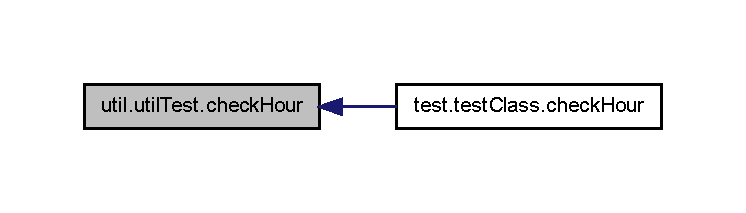
\includegraphics[width=358pt]{classutil_1_1util_test_a778f4f1a2c59966aa2aae9011bde2ca8_icgraph}
\end{center}
\end{figure}


\hypertarget{classutil_1_1util_test_a0511fb76ddd99ce9c98231108be97d5a}{
\index{util::utilTest@{util::utilTest}!checkString@{checkString}}
\index{checkString@{checkString}!util::utilTest@{util::utilTest}}
\subsubsection[{checkString}]{\setlength{\rightskip}{0pt plus 5cm}static boolean util.utilTest.checkString (
\begin{DoxyParamCaption}
\item[{String}]{ s}
\end{DoxyParamCaption}
)\hspace{0.3cm}{\ttfamily  \mbox{[}static\mbox{]}}}}
\label{classutil_1_1util_test_a0511fb76ddd99ce9c98231108be97d5a}


checkString Metodo que verifica si un String pasado como parametro es valido o no. Un string es valido si solo contiene caracteres de a-\/z o de A-\/Z y ademas si su longitid esta entre 1 y 60. 


\begin{DoxyParams}{Parameters}
{\em String} & s es el string a verificar. \\
\hline
\end{DoxyParams}
\begin{DoxyReturn}{Returns}
boolean true si es valido y false en caso contrario. 
\end{DoxyReturn}


Here is the caller graph for this function:
\nopagebreak
\begin{figure}[H]
\begin{center}
\leavevmode
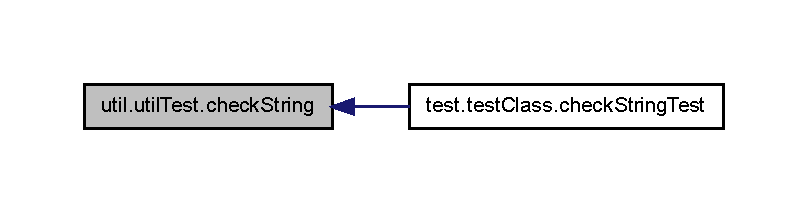
\includegraphics[width=388pt]{classutil_1_1util_test_a0511fb76ddd99ce9c98231108be97d5a_icgraph}
\end{center}
\end{figure}


\hypertarget{classutil_1_1util_test_a9e7d593af72519ead8d188becaa1c671}{
\index{util::utilTest@{util::utilTest}!daysDiff@{daysDiff}}
\index{daysDiff@{daysDiff}!util::utilTest@{util::utilTest}}
\subsubsection[{daysDiff}]{\setlength{\rightskip}{0pt plus 5cm}static int util.utilTest.daysDiff (
\begin{DoxyParamCaption}
\item[{int}]{ diaE, }
\item[{int}]{ mesE, }
\item[{int}]{ anioE, }
\item[{int}]{ hsE, }
\item[{int}]{ minE, }
\item[{int}]{ diaS, }
\item[{int}]{ mesS, }
\item[{int}]{ anioS, }
\item[{int}]{ hsS, }
\item[{int}]{ minS}
\end{DoxyParamCaption}
)\hspace{0.3cm}{\ttfamily  \mbox{[}static\mbox{]}}}}
\label{classutil_1_1util_test_a9e7d593af72519ead8d188becaa1c671}
daysDiff permite calcular la cantidad de d�as que un paciente ha estado internado. A partir de las 10:00 de la ma�ana ya se considera un nuevo d�a, es decir, si el paciente es dado de alta a las 10:01 ya se le cobra un nuevo d�a. 
\begin{DoxyParams}{Parameters}
{\em int} & diaE representa al dia de inicio. \\
\hline
{\em int} & mesE representa al mes de inicio. \\
\hline
{\em int} & anioE representa al anio de inicio. \\
\hline
{\em int} & hsE representa a la hs de inicio. \\
\hline
{\em int} & minS representa a los minutos de fin. \\
\hline
{\em int} & diaS representa al dia de fin. \\
\hline
{\em int} & mesS representa al mes de fin. \\
\hline
{\em int} & anioS representa al anio de fin. \\
\hline
{\em int} & hsS representa a la hs de fin. \\
\hline
{\em int} & minS representa a los minutos de fin. \\
\hline
\end{DoxyParams}
\begin{DoxyReturn}{Returns}
float representando la cantidad de dias de internacion que se le deben cobrar al paciente. 
\end{DoxyReturn}


Here is the call graph for this function:
\nopagebreak
\begin{figure}[H]
\begin{center}
\leavevmode
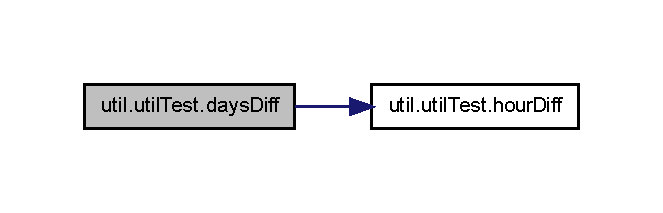
\includegraphics[width=318pt]{classutil_1_1util_test_a9e7d593af72519ead8d188becaa1c671_cgraph}
\end{center}
\end{figure}




Here is the caller graph for this function:
\nopagebreak
\begin{figure}[H]
\begin{center}
\leavevmode
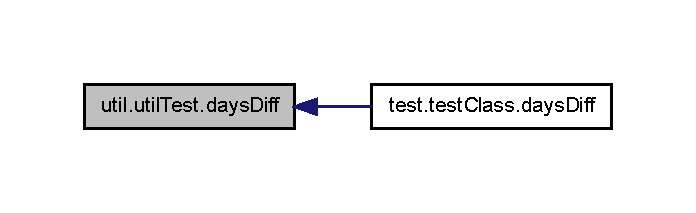
\includegraphics[width=334pt]{classutil_1_1util_test_a9e7d593af72519ead8d188becaa1c671_icgraph}
\end{center}
\end{figure}


\hypertarget{classutil_1_1util_test_aaa8556f9ef98f63b750e50af6c3484d1}{
\index{util::utilTest@{util::utilTest}!hourDiff@{hourDiff}}
\index{hourDiff@{hourDiff}!util::utilTest@{util::utilTest}}
\subsubsection[{hourDiff}]{\setlength{\rightskip}{0pt plus 5cm}static int util.utilTest.hourDiff (
\begin{DoxyParamCaption}
\item[{int}]{ diaE, }
\item[{int}]{ mesE, }
\item[{int}]{ anioE, }
\item[{int}]{ hsE, }
\item[{int}]{ minE, }
\item[{int}]{ diaS, }
\item[{int}]{ mesS, }
\item[{int}]{ anioS, }
\item[{int}]{ hsS, }
\item[{int}]{ minS}
\end{DoxyParamCaption}
)\hspace{0.3cm}{\ttfamily  \mbox{[}static\mbox{]}}}}
\label{classutil_1_1util_test_aaa8556f9ef98f63b750e50af6c3484d1}
hourDiff indica la cantidad de horas la cantidad de horas transcurridas entre dos fechas (fecha y hora). 
\begin{DoxyParams}{Parameters}
{\em int} & diaE representa al dia de inicio. \\
\hline
{\em int} & mesE representa al mes de inicio. \\
\hline
{\em int} & anioE representa al anio de inicio. \\
\hline
{\em int} & hsE representa a la hs de inicio. \\
\hline
{\em int} & minS representa a los minutos de fin. \\
\hline
{\em int} & diaS representa al dia de fin. \\
\hline
{\em int} & mesS representa al mes de fin. \\
\hline
{\em int} & anioS representa al anio de fin. \\
\hline
{\em int} & hsS representa a la hs de fin. \\
\hline
{\em int} & minS representa a los minutos de fin. \\
\hline
{\em int} & anio representa el anio a chequear. \\
\hline
\end{DoxyParams}
\begin{DoxyReturn}{Returns}
int que representa la cantidad de horas que hay entre 2 fechas. 
\end{DoxyReturn}


Here is the caller graph for this function:
\nopagebreak
\begin{figure}[H]
\begin{center}
\leavevmode
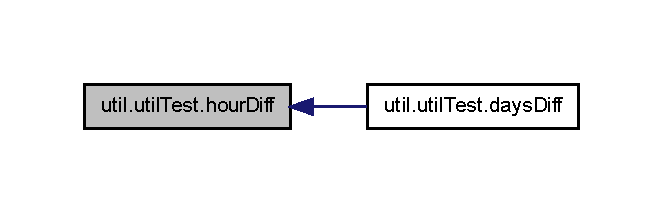
\includegraphics[width=400pt]{classutil_1_1util_test_aaa8556f9ef98f63b750e50af6c3484d1_icgraph}
\end{center}
\end{figure}


\hypertarget{classutil_1_1util_test_a991f47fa2395bca0ddc28abb2ca2950f}{
\index{util::utilTest@{util::utilTest}!medicPay@{medicPay}}
\index{medicPay@{medicPay}!util::utilTest@{util::utilTest}}
\subsubsection[{medicPay}]{\setlength{\rightskip}{0pt plus 5cm}static float util.utilTest.medicPay (
\begin{DoxyParamCaption}
\item[{Vector$<$ {\bf Pair} $>$}]{ consultas, }
\item[{float}]{ valor, }
\item[{int}]{ horasAlquiler, }
\item[{float}]{ alquilerxhs}
\end{DoxyParamCaption}
)\hspace{0.3cm}{\ttfamily  \mbox{[}static\mbox{]}}}}
\label{classutil_1_1util_test_a991f47fa2395bca0ddc28abb2ca2950f}
Una funci�n que permita calcular el sueldo de un m dico en funci�n de la cantidad de\par
 consultas atendidas al mes, las obras sociales y el valor de la consulta. A este\par
 resultado se le deber� descontar la cantidad de horas que el profesional\par
 ha utilizado la cl�nica(en concepto de alquiler). 
\begin{DoxyParams}{Parameters}
{\em consultas} & \\
\hline
{\em valor} & \\
\hline
{\em horasAlquiler} & \\
\hline
{\em alquilerxhs} & \\
\hline
\end{DoxyParams}
\begin{DoxyReturn}{Returns}
pago 
\end{DoxyReturn}


Here is the caller graph for this function:
\nopagebreak
\begin{figure}[H]
\begin{center}
\leavevmode
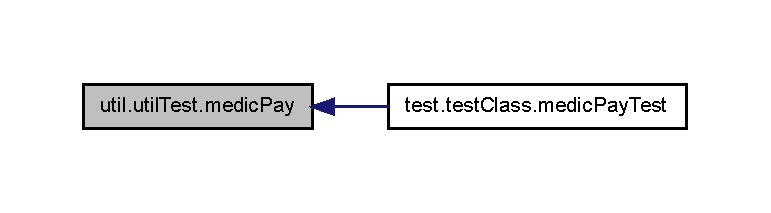
\includegraphics[width=370pt]{classutil_1_1util_test_a991f47fa2395bca0ddc28abb2ca2950f_icgraph}
\end{center}
\end{figure}


\hypertarget{classutil_1_1util_test_a525d627e3d989ff9190a69fe6bccffff}{
\index{util::utilTest@{util::utilTest}!totalPay@{totalPay}}
\index{totalPay@{totalPay}!util::utilTest@{util::utilTest}}
\subsubsection[{totalPay}]{\setlength{\rightskip}{0pt plus 5cm}static float util.utilTest.totalPay (
\begin{DoxyParamCaption}
\item[{Float}]{ costoDia, }
\item[{{\bf Pair}\mbox{[}$\,$\mbox{]}}]{ comidas, }
\item[{Vector$<$ {\bf Pair} $>$}]{ medicamentos, }
\item[{int}]{ dias, }
\item[{Float}]{ descuento}
\end{DoxyParamCaption}
)\hspace{0.3cm}{\ttfamily  \mbox{[}static\mbox{]}}}}
\label{classutil_1_1util_test_a525d627e3d989ff9190a69fe6bccffff}
Una funci�n que permita calcular el monto total que debe abonar un paciente\par
 internado en funci�n del costo del d�a de internaci�n, cantidad y costos de comidas\par
 recibidas, cantidad y costo de medicamentos recibidos. A todo esto debe calcularse un\par
 descuento correspondiente al monto que cubre la mutual. 
\begin{DoxyParams}{Parameters}
{\em costoDia} & \\
\hline
{\em comidas} & \\
\hline
{\em medicamentos} & \\
\hline
{\em dias} & \\
\hline
{\em descuento} & \\
\hline
\end{DoxyParams}
\begin{DoxyReturn}{Returns}
monto 
\end{DoxyReturn}


Here is the caller graph for this function:
\nopagebreak
\begin{figure}[H]
\begin{center}
\leavevmode
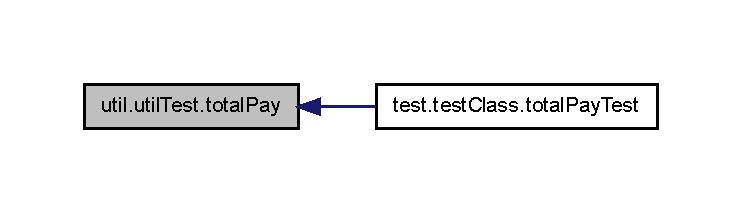
\includegraphics[width=356pt]{classutil_1_1util_test_a525d627e3d989ff9190a69fe6bccffff_icgraph}
\end{center}
\end{figure}




The documentation for this class was generated from the following file:\begin{DoxyCompactItemize}
\item 
src/util/\hyperlink{util_test_8java}{utilTest.java}\end{DoxyCompactItemize}

\chapter{Documentación de archivos}
\hypertarget{test_class_8java}{
\section{src/test/testClass.java File Reference}
\label{test_class_8java}\index{src/test/testClass.java@{src/test/testClass.java}}
}


Este archivos contiene la implementacion de las pruebas.  


\subsection*{Classes}
\begin{DoxyCompactItemize}
\item 
class \hyperlink{classtest_1_1test_class}{test.testClass}
\begin{DoxyCompactList}\small\item\em La clase \hyperlink{classtest_1_1test_class}{testClass} declara una serie de metodos en jUnit\par
 para verficar el correcto funcionamiento de las funciones de validacion\par
 de la clase utilTest.\par
 \item\end{DoxyCompactList}\end{DoxyCompactItemize}


\subsection{Detailed Description}
Este archivos contiene la implementacion de las pruebas. \begin{DoxyAuthor}{Author}
BERNAL, Matias\par
 BRESSAN, Gonzalo\par
 JAULE, Marcos\par
 ODORIZZI, Eduardo
\end{DoxyAuthor}
\begin{DoxyDate}{Date}
November, 1st 2010 
\end{DoxyDate}

\section{Referencia del Archivo src/util/Pair.java}
\label{_pair_8java}\index{src/util/Pair.java@{src/util/Pair.java}}


Este archivo contiene la impementaci\'{o}n del tipo Par.  


\subsection*{Clases}
\begin{DoxyCompactItemize}
\item 
class {\bf util.Pair}
\begin{DoxyCompactList}\small\item\em La clase pair implementa el tipo Par. \item\end{DoxyCompactList}\end{DoxyCompactItemize}


\subsection{Descripción detallada}
Este archivo contiene la impementaci\'{o}n del tipo Par. \begin{DoxyAuthor}{Autor}
BERNAL, Matias\par
 BRESSAN, Gonzalo\par
 JAULE, Marcos\par
 ODORIZZI, Eduardo
\end{DoxyAuthor}
\begin{DoxyDate}{Fecha}
November, 1st 2010 
\end{DoxyDate}

\hypertarget{util_test_8java}{
\section{src/util/utilTest.java File Reference}
\label{util_test_8java}\index{src/util/utilTest.java@{src/util/utilTest.java}}
}


This file contains the DoxygenExample class with the main() function.  


\subsection*{Classes}
\begin{DoxyCompactItemize}
\item 
class \hyperlink{classutil_1_1util_test}{util.utilTest}
\begin{DoxyCompactList}\small\item\em La clase \hyperlink{classutil_1_1util_test}{utilTest} declara una serie de metodos para realizar validaciones de, entre otros,\par
 Cadenas, Fechas, Tiempo transcurrido. \item\end{DoxyCompactList}\end{DoxyCompactItemize}


\subsection{Detailed Description}
This file contains the DoxygenExample class with the main() function. \begin{DoxyAuthor}{Author}
BERNAL, Matias\par
 BRESSAN, Gonzalo\par
 JAULE, Marcos\par
 ODORIZZI, Eduardo
\end{DoxyAuthor}
\begin{DoxyDate}{Date}
November, 1st 2010 
\end{DoxyDate}

\printindex
\end{document}
